\section{Clustering}
This section explains the various clustering algorithms used in the research.
Subsequently, we will explain and indicate how the hyperparameters are handled in the research for each algorithm.
\subsection{Types of clustering algorithms}
Multiple clustering types can be utilized for clustering data \citep{xu_comprehensive_2015}.
For this study, we selected the types that use some form of distance for clustering.
We explain each cluster type with corresponding clustering algorithms.
\subsubsection{Partition based clustering}
With this type, the data is partitioned and allocated into a fixed amount of clusters.
A well-known and popular clustering algorithm is K-means.
Based on Loyd et al.'s original method, this algorithm randomly selects $k$ points as cluster centroids \citep{1056489}.
The first step of the algorithm is to assign each datapoint $x_i$ to the nearest centroid.
Then the mean is calculated by calculating the mean of all points in the cluster \citep{yuan_research_2019}:
\begin{equation}
    c_i = \frac{1}{|C_i|} \sum_{x_i \in C_i} x_i
\end{equation}
Finally, the K-Means algorithm aims to minimize the within-cluster sum of squares (WCSS) \citep{yuan_research_2019}:
\begin{equation}
    WCSS = \sum_{i=1}^{k} \sum_{c_i \in C_i} || x_i, c_i ||^2
\end{equation}
The algorithm runs multiple times until the center point no longer changes or reaches the maximum iterations \citep{yuan_research_2019}.

%Iteratively each data point is assigned to its nearest centroid.
%It keeps proceeding until the distance between the cluster centroids is optimal.
%The algorithm can also be used in a distributed manner.
%Instead of calculating the centroids locally, each party receives the centroids and calculates their nearest centroids [Xia et al., 2020].
%Although K-means serves its purpose well, it requires pre-defining the number of clusters and is sensitive to outliers \citep{keller_balancing_2021}.
%Therefore, a parameterless alternative to K-means is \gls{ap} \citep{frey_clustering_2007}.

%\gls{ap} is an algorithm that clusters data points by iteratively passing messages between them.
%Each point sends and receives messages about the attractiveness of other points as cluster centers (exemplars) and the suitability of itself as a center \citep{keller_balancing_2021}.

\subsubsection{Density based clustering}
The data points are partitioned for this clustering type based on nearest neighbors \citep{fahad_survey_2014}.
A region with a high data density is considered a cluster \citep{xu_comprehensive_2015}.
A popular density-based clustering algorithm is \gls{dbscan}.
The method was introduced by Ester et al. and worked by drawing a radius around data points \citep{ester_density-based_nodate}.
For this thesis, the $\Pi$-symbol is used not to confuse it with the privacy budget $\epsilon$.
It then groups all points within this radius as clusters.
The main advantage is its ability to find arbitrarily shaped clusters and detect outliers \citep{liu_privacy_2012}.

Another density-based algorithm is \gls{optics}, an extension of \gls{dbscan}.
The algorithm attempts different $\Pi$ values to achieve the best result \citep{ankerst_optics_nodate}.
The algorithm uses \gls{dbscan}, so we explain this algorithm first in detail.
It calculates the "density-reachable" property of each data point first \citep{ankerst_optics_nodate}:
\begin{equation}
    N_Pi(x_i) = {x_i \in X : d(x_i, x_j) \leq \Pi}
\end{equation}
If $N_Pi(x_i) \geq minPts$ then $x_i$ is a "core-object" \citep{ankerst_optics_nodate}.
These core objects are used for identifying dense regions to grow clusters.
Second is the "density-connected" property, where two points can be linked through a series of points close to each other (within distance $\Pi$).
And, each has a sufficient number of neighbors ($minPts$) \citep{ankerst_optics_nodate}.
The final step is to build clusters based on these two properties.
A cluster $C$ is build up using the following rules \citep{ankerst_optics_nodate}:
\begin{enumerate}
    \item If a core-object in $C$ is density-reachable from $x_i$, $\Pi$ and $minPts$. Then $x_i$ is added to $C$.
    \item If a core-object is density-connected to $x_i$, $\Pi$ and $minPts$. Then $x_i$ is added to $C$.
\end{enumerate}
Finally, \gls{optics} comes into play, which makes the radius $\Pi$ obsolete.
Instead of constructing clusters, the \gls{optics} algorithm produces an ordered list.
In the next step, they create a reachability plot that shows valleys (clusters) and peaks (cluster transitions).
The algorithm then uses an automatic approach to determining the characteristics of the reachability plot to determine clusters.
\mycomment{
    Instead of directly assigning data points to clusters, specific distance calculations are stored in a list.
    For each data point, it tracks two values: core distance and reachability distance.
    These values represent the shortest distance to make a data point, $p$, a core point, and the shortest distance from $p$ to another core point, $p'$, respectively.
    A specific ordering is maintained to ensure that clusters with higher density values are processed first.
    Based on this ordering, \gls{optics} constructs the \gls{dbscan} algorithm hierarchically \citep{schubert_dbscan_2017}.
    \todo[inline]{better to bring formal definition rather than text for all clustering algorithms that are used in your text}}

\subsubsection{Hierarchical clustering}
%The name originates from the way hierarchical clustering works.
A hierarchy of clusters is generated and merged according to the closeness of data points \citep{meng_private_2021}. Because this is structured as a tree, it can be described using a binary tree and visualised with a dendogram  \citep{nielsen_hierarchical_2016}.
Hierarchical clustering can be divided into agglomerative and divisive \citep{meng_private_2021}.
This approach means the clustering occurs from the bottom-up or top-down, respectively.
Of the two approaches, agglomerative is the most common one \citep{meng_private_2021}.
For  agglomerative definition, we consider the following definition:
\begin{equation}
    L(C_i, C_j) = min_{x \in C_i, y \in C_j} d(x, y)
\end{equation}
\begin{enumerate}
\item Initially, each data-point $x \in X$ is treated as its own cluster \citep{nielsen_hierarchical_2016}.
    \item Merge $C_i$ and $C_j$ based on a certain metric, and add $C_{ij}$ to the list and remove $C_i$ and $C_j$ from the list \citep{nielsen_hierarchical_2016}.
    \item The final cluster should contain all the data points, which is the dendogram root ($C_{root} = X$) \citep{nielsen_hierarchical_2016}.
\end{enumerate}
The specific implementation and calculation of the closeness of data-points, depends on the linkage function.
For this function, there are four popular options: Single link, Average link, Complete link, and Ward's method \citep{roux_comparative_2015}. In the next section we evaluate this to choose the most fitting option.

\subsubsection{Research direction}
There are three different types of clustering algorithms that we have considered for this research.
Therefore, we will choose one algorithm for each type to ensure a representative selection.

Based on the different types of clustering algorithms, we have chosen to use K-Means for this research.
K-Mean clustering is widely used in the literature and, therefore, easily compared with other studies.

For density-based clustering, we will solely focus on \gls{optics} in this study.
The parameter $\Pi$ in \gls{dbscan} is influenced by the data shape, which is further affected by our privacy mechanism.
However, as \gls{optics} automatically determines the $\Pi$, the impact of this parameter is less significant, enabling us to emphasize the evaluation of the privacy mechanism itself.

As for hierarchical clustering, we have decided to go for agglomerative clustering.
%Because the \gls{dbscan}'s $epsilon'$ algorithm is sensitive to the shape $epsilon'$ value, we utilize \gls{optics} for this research instead of \gls{dbscan}.

%Another density-based cluster method is Density Peak Clustering (DPC). 
%The algorithm calculates the local density of each data point and identifies density peaks for points with the highest density [Rodriguez and Laio, 2014].

\subsection{Parameter selection}
A list of important hyper parameters that can influence the results is provided for each clustering algorithm.
Subsequently, we briefly discuss the methods for determining these hyper parameters for the algorithms. \newline
We use the same distance function for all algorithms to have all the algorithms in the same setting.
This function will be Euclidean distance, as used for \gls{gi}.
\subsubsection{K-Means} \label{theory:kmeans}
The most crucial parameter of the K-Means algorithm is the value of $k$.
This value determines the number of clusters to consider and influences the results by a lot \citep{ahmed_k-means_2020}.
%These methods require a manual way of selecting the best $k$ by visual inspection of a plot.
The first method is called an "elbow" plot \citep{kodinariya_review_2013}.
This method finds the best $k$ by applying the K-Means algorithm multiple times and estimating the best $k$.
Based on the line's visual change, someone can select the best $k$:
\begin{figure}[H]
    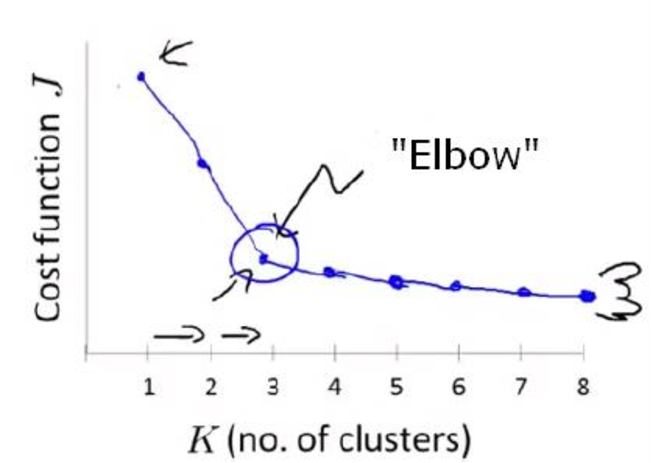
\includegraphics{TheorethicalFramework/dentification-of-Elbow-point.png}
    \caption{Illustration of determining $k$ using the "elbow" method \citep{kodinariya_review_2013}}
    \label{elbow-method}
\end{figure}
The cost function $J$ on the y-axis is a metric to measure cluster distance/cohesion \citep{yuan_research_2019}.
Because there has to be a clear "elbow", using the "distortion" metric is the most straightforward \citep{yuan_research_2019}. This is the Sum of square errors (SSE), and because this value reduces for a higher amount of clusters; there is a distinctive curve as visualized in Figure \ref{elbow-method}. 

Another good option for determining $k$ is the silhouette coefficient, as this metric measures the separation and cohesion of the cluster, it can be used to choose an optimal amount of clusters \citep{saputra_effect_2020}. The method is related to the "elbow" plot by plotting a line, but now the highest value is selected instead of the "elbow":
\begin{figure}
    \centering
    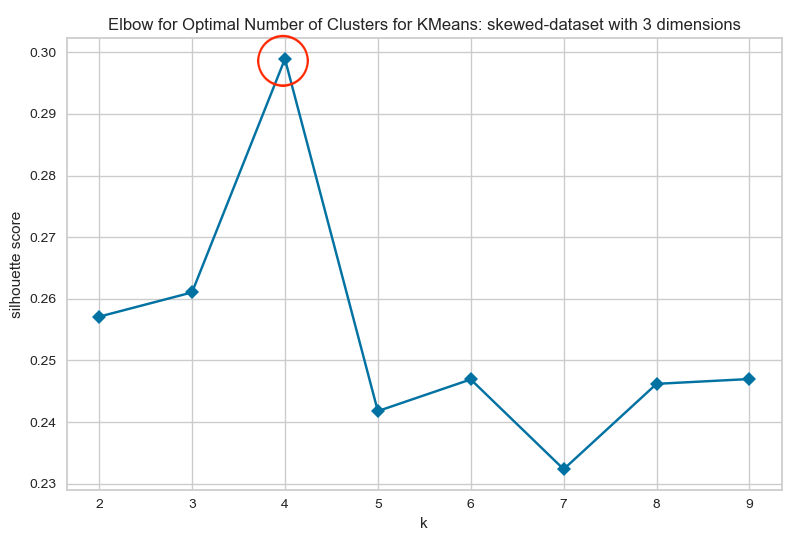
\includegraphics[width=0.75\linewidth]{skewed-dataset-3-kmeans.png}
    \caption{An example on how to select the best (red circle) silhouette score, using the silhouette plot method \citep{saputra_effect_2020}}
    \label{fig:k-select-silhouette}
\end{figure}

\newline
A final metric to consider is the Gap statistic method \citep{yuan_research_2019}.
It compares the total within-cluster variation for different values of $k$ with their expected values under a null reference distribution of the data \citep{tibshirani_estimating_2001}.

The silhouette coefficient and gap statistic methods are robust, but are performance intensive for bigger data-sets \citep{yuan_research_2019}. Where the Gap statistic is the slowest from the three, and SSE the fastest.
On the other hand, the SSE can be hard to interpreted as the "elbow" is not always visible \citep{yuan_research_2019}}. Also, the SSE only calculates the distance information, while the other two metrics also incorporate other indicators.

Although performance is important, the data-sets that are used in this thesis are not relatively small. However, the time complexity of Gap statistic is a lot higher then Silhouette plot, while the results are comparable \citep{yuan_research_2019}. Therefore, we decided to go for the Silhouette Coefficient method. The formal definition is provided in the next Section: \ref{eq:silhouette_coefficient}.

\subsubsection{Agglomerative Clustering} \label{theory:clustering-agglomerative}
The agglomerative clustering algorithm has two essential hyper parameters: the linkage method and the number of clusters. \newline
\textbf{Choosing linkage:}
This decision is crucial for the algorithm as it determines the similarity measurement.
Choosing a linkage method that uses Euclidean distance is important for our research.
From the four different types of linkage methods, we have chosen the Ward method because this method uses Euclidean distance \citep{roux_comparative_2015,seetharaman_brief_2019}. \newline
\textbf{Choosing number of clusters:}
There are not many methods for determining the initial number of clusters.
Therefore, the approach is similar to K-Means.
The amount of clusters is selected based on the silhouette method, by selecting the highest silhouette score for a given $k$.

\mycomment{\subsubsection{Affinity Propagation} \label{theory:clustering-ap}
    %\gls{ap} is an algorithm that clusters data points by iteratively passing messages between them.
    %Each point sends and receives messages about the attractiveness of other points as cluster centers (exemplars) and the suitability of itself as a center \citep{keller_balancing_2021}.
    %The method was introduced by Frey et al. and does not require any hyperparameters \citep{frey_clustering_2007}.
    Although the algorithm is parameter-less, important properties could potentially impact the clustering \citep{wang_adaptive_2007}. \newline
    \textbf{Choosing preference($p$): }
    Indicates the preference for selecting a data point as cluster center \citep{wang_adaptive_2007}.
    It highly influences the number of clusters; a high one would lead to more clusters and a small one to less \citep{moiane_evaluation_2018}.
    Depending on the data, a good choice is to set the $p$ to the median of all data similarities \citep{wang_adaptive_2007}.
    But, the effectiveness of this could be highly influenced based on the dataset.
    Analyzing the silhouette coefficient \citep{moiane_evaluation_2018} to validate if the preference is correctly set is possible.
    \newline
    \textbf{Choosing damping factor($lam \in [0,1] $):}
    The damping factor improves the stability (convergence) of the algorithm \citep{wang_adaptive_2007}.
    By default, this value is 0.5 and can be increased to 1 to reduce the impact of numerical oscillations.
    This value can be found manually by re-running the algorithm to find the optimal value.
    However, the approach takes a lot of time, especially for bigger datasets \citep{wang_adaptive_2007}. \newline

    To conclude on this, damping is important if big datasets are considered.
    %However, this research does not use large datasets or consider time complexity as a metric.
    On the other hand, the preference could influence the results a lot.
    In general, it should be sufficient to take the median.
}
\subsubsection{OPTICS} \label{theory:clustering-dbscan}
With the introduction of \gls{optics}, we no longer need to worry about the $radius(\epsilon)$ value.
Therefore, only $minPts$ remains an important parameter to consider. \newline
%\todo[inline]{Use OPTICS instead of DBSCAN}
%\gls{dbscan} is introduced by \citep{ester_density-based_nodate} and draws a radius (neighborhood) around data points.
%It then groups all points within this radius as clusters. The main advantage is its ability to find arbitrarily shaped clusters and detect outliers \citep{liu_privacy_2012}.
%The \gls{dbscan} algorithm uses the inputs $minPts$, $radius(\epsilon)$ (not to be confused with the privacy budget $\epsilon$), and the Euclidean distance \citep{schubert_dbscan_2017}.
%This $\epsilon'$ is used to draw a neighborhood, and the $minPts$ is used as a weight to evaluate which points should be inside the neighborhood.
%The Euclidean distance is used for the distance function to be consistent with the other algorithms. \newline
The $minPts$ is the minimum amount of points that have to be within the $radius(\epsilon)$ to mark it a cluster.
This hyperparameter is analyzed in a paper by Sander et al.
The work describes calculating this parameter by applying two times the feature amount \citep{sander_density-based_1998}.
So, using this approach, a dataset with two features will have an $minPts$ of four \citep{schubert_dbscan_2017}.

\mycomment{\textbf{Choosing radius($\epsilon'$):} The desired $\epsilon'$ can be calculated using the K-NearestNeighbours algorithm \citep{ester_density-based_nodate,schubert_dbscan_2017}.
    The general approach is to choose a $K = 2*N - 1$ (where N is the number of features) and plot the distance for each point.
    This can then be plotted using a k-dist plot, and the best "elbow" can be chosen for deciding the $\epsilon$ (similar to choosing the $k$ for K-means) \citep{elbatta_dynamic_2013}.
    \begin{figure}[H]
        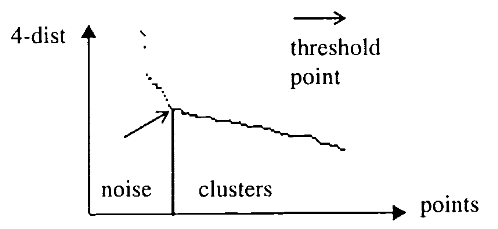
\includegraphics{TheorethicalFramework/K-dist-elbow.png}
        \caption{K-dist plot example for $minPts = 4$ based on a 2-dimensional dataset \citep{ester_density-based_nodate}}
        \label{k-dist-plot}
    \end{figure}

    %The epsilon value is crucial for the DBSCAN algorithm and highly dependent on the dataset \todo{Source}.
    Since we employ various types of datasets and algorithms, it is desirable to have an automated method for determining the epsilon (radius) value.
    The epsilon could influence the results as the radius determines the clusters.
    For this reason, research has also been conducted on an extension of DBSCAN called OPTICS.}

%In conclusion, K-Means and \gls{ap} have straightforward methods for determining hyperparameters.
%For K-Means, the elbow method is the most common, and for \gls{ap}, the median is used for the preference.
\gls{dbscan} is a little more complicated due to the variety of datasets and noise-altering mechanisms we experiment with.
This complexity is why we use \gls{optics} to determine the best value for $radius(\epsilon)$ and choose $minPts$ based on the number of features times two.

\mycomment{\subsection{Overfitting}
    Overfitting is dangerous for machine learning models and one of the biggest mistakes with training machine learning models \citep{demsar_hands-training_2021}.
    It occurs when a machine learning model is trained on samples that are not representative of future test data \citep{bashir_information-theoretic_2020}.
    A common mistake is to evaluate a model using the same data as it is trained on \citep{demsar_hands-training_2021}.
    The model appears to have high accuracy but just memorized the properties of a training dataset.
    Another cause of overfitting can be the size of the training data \citep{valdenegro-toro_machine_2022}.

    To measure if a model overfits, it is necessary to compute the generalization gap \citep{valdenegro-toro_machine_2022}.
    \begin{equation}
        L_{gap} = L_{val} - L_{train}
    \end{equation}
    Where $L{val}$ and $L_{train}$ are the validation and training splits of the dataset.
    For splitting a dataset, a common approach is to have 50\% training data, 30\% for validation and 20\% test \citep{chicco_ten_2017}.
    In addition to this, if a dataset is too small cross-validation can be considered.

    \todo[inline]{Needs more work for unsupervised / cluster problems}

    In summary:
    \begin{enumerate}
        \item It is necessary to evaluate a machine learning model on a dataset that was not used to train the model.
        \item Use a representative training dataset, to work well on unseen data.
        \item To reduce the chance of overfitting for supervised learning, it is a good practice to validate using a 30\% subset.
    \end{enumerate}
}

\subsection{Evaluation methods} \label{theory:evaluate}
Clustering comparison measures are important in cluster analysis for external validation by comparing clustering solutions to a "ground truth" clustering \citep{vinh_information_nodate}.
These external validity indices are a common way to assess the quality of unsupervised machine learning methods like clustering \citep{warrens_understanding_2022}.
A method that could be used for this is the Rand Index \citep{rand_objective_1971}.
It is a commonly applied method for comparing two clustering algorithms \citep{wagner_comparing_nodate}.
An improvement of this method is adjusted for chance by considering the similarity of pairwise cluster comparisons \citep{vinh_information_nodate}.
Both the Rand Index (RI) and Adjusted Rand Index (ARI) \citep{hubert_comparing_1985} report a value between 0 and 1.
Where 0 is for no-similarity and 1 for identical clusters.
Alternatives for RI are the Fowles-Mallows Index and Mirkin Metric.
However, these two methods have their disadvantages. They are, respectively, sensitive to a few clusters and cluster sizes \citep{wagner_comparing_nodate}.
The ARI metric suffers from cluster size imbalance as well, so it only provides not a lot of information on smaller clusters \citep{warrens_understanding_2022}.
Instead, they recommend using the cluster index metric proposed by Fränti et al. \citep{franti_centroid_2014}.

Another popular group of methods is the information theoric-based measures \citep{vinh_information_nodate}.
This metric measures the information between centroids; the higher the value, the better \citep{vinh_information_nodate}.
\gls{mi} is a metric that calculates the probability of an element belonging to cluster $C$ or $C`$.
But, it is not easy to interpret as it does not have a maximum value \citep{wagner_comparing_nodate}.
To this end, \gls{nmi} can be used to report a value between 0 and 1 using the geometric mean \citep{strehl_cluster_2002}.
The metric also exists in an adjusted version as \gls{ami}.
This metric works in the same way as for the \gls{ari} and is mainly needed if the number of data items is small in comparison to the number of clusters \citep{vinh_information_nodate}. \newline

Besides the external validity measurements for clustering, it is also possible to use internal validation methods.
These metrics focus entirely on the intrinsic dataset properties instead of relying on an external baseline clustering algorithm \citep{craenendonck_using_nodate}.
They are assessing two essential concepts of clustering: compactness and separation \citep{hassani_using_2017}.
Both studies consider three different metrics and measure both concepts at the same time \citep{hassani_using_2017}:
\begin{enumerate}
    \item \gls{chi} \citep{calinski_dendrite_1974} is used to measure the cluster variance (well-separated clusters) and low variance within the clusters (tightly coupled data). A high score indicates better clustering.
    \item \gls{sc} \citep{rousseeuw_silhouettes_1987} This metric is similar in measuring cohesion within and separating clusters.
          However, this metric uses the pairwise distance \citep{hassani_using_2017}.
          A score of -1 indicates incorrect clustering and +1 for correct clustering \citep{rousseeuw_silhouettes_1987}.
    \item Davies-Bouldin (DB) \citep{davies_cluster_1979} uses the average distance between clusters. A lower score indicates good clustering.
\end{enumerate}

%K-Means scores relatively high for \gls{chi} \citep{craenendonck_using_nodate,hassani_using_2017} and \gls{sc} \citep{craenendonck_using_nodate}.
%The same applies to \gls{optics}/\gls{dbscan}, which scores relatively high on \gls{sc} and DB due to noise sensitivity \citep{craenendonck_using_nodate}.

% Thus, these metrics are difficult to use for very different clustering algorithms \cite{craenendonck_using_nodate}.
\mycomment{\subsubsection{Existing literature}
    \todo[inline]{What to do with this? it seems he beginning of this section you already presented some literature studies; it is a bit confusing to bring the literature two times}
    %A recent and much-cited study uses \gls{ari} and accuracy as metrics for evaluating K-Means \cite{ahmed_k-means_2020}.
    %The accuracy is measured by calculating the percentage of the correct predicted labels and their truth labels.
    Comparable studies with differential privacy use external validation \citep{xia_distributed_2020, sun_privbv_2022}.
    Their experiment setup uses a so-called non-private clustering algorithm as external validation.
    This clustering algorithm is trained without the perturbed data and compared with the same clustering algorithm trained with perturbed data.
    Thus, the non-private variant provides the ground truth as an external validation.

    They compare the mutual information between a baseline clustering algorithm using \gls{ami} \citep{9679364} or \gls{nmi} \citep{xia_distributed_2020,sun_privbv_2022}.
    Another study for evaluating \gls{dp} with \gls{ap} uses both \gls{ari} and \gls{ami}.
    In addition to mutual information and rand index scores, it is also not uncommon to calculate the error between the two clustering algorithm's centroids \citep{xia_distributed_2020, 9679364}.
    These two studies used Relative Error (RE) for this.}

\subsubsection{Research direction}
This chapter outlines the evaluation methods used and provides a definition and brief explanation for each method.

In the literature, both internal and external evaluation methods are commonly used.
While some studies choose one over the other, this thesis will perform both validations.
This approach is crucial to measure how well the data shape is preserved (internal validation) and how the algorithm performs in real-world scenarios (external validation).
Our research will focus on \gls{ami} for external validation. Because it holds the same value as \gls{ari}, but it is better explainable.
The second metric we use is for external validation. We use \gls{sc} because this metric returns a bounded value between -1 and 1.

%Since certain clustering algorithms may score higher or lower on specific metrics, it is essential to choose two metrics for each type of validation.
Based on existing studies and the literature, we have selected metrics adjusted to compensate for the data distribution characteristics.
Hence, we will focus on these metrics' "adjusted" variants:
\begin{enumerate}
    \item \textbf{Silhouette coefficient (Internal validation): \label{eq:silhouette_coefficient}}
          \mycomment{\item \textbf{Calinski Harabasz Index:}
          The definition of \gls{chi} is defined in several steps \citep{liu_understanding_2010}:
          The first definition is the between cluster sum of squares.
          \begin{equation}
              B = \sum_{i=1} n_i \cdot (C_k - C)^2
          \end{equation}
          \begin{enumerate}
              \item $n_k$ is the number of data points in cluster $k$.
              \item $C_k$ is the centroid of cluster $k$.
              \item $C$ is the dataset centroid
          \end{enumerate}
          The second part of the definition is defined as follows:
          \begin{equation}
              W_k = \sum_{i=1}n_i \cdot (x_i - C_k)^2
          \end{equation}
          $W_k$ is the within-cluster sum of squares and $x_i$ is the $i$th data point.
          Finally, the \gls{chi} is calculated by combining the between and within-cluster calculations:
          \begin{equation}
              CH = \frac{B}{\sum_{k=1}^{K}} \cdot \frac{N - k}{k - 1}
          \end{equation}
          \begin{enumerate}
              \item $K$ is the number of clusters.
              \item $N$ is the number of data points.
          \end{enumerate}}

          This metric is defined as follows \citep{liu_understanding_2010,rousseeuw_silhouettes_1987}:
          \begin{equation}
              s(i) = \frac{b(i) - a(i)}{max(b(i) - a(i))}
          \end{equation}
          \begin{enumerate}
              \item $s(i)$ is the silhouette coefficient for a single datapoint $i$.
              \item $a(i)$ is the mean distance of $i$ and all the other points in the same cluster.
              \item $b(i)$ is the mean distance of $i$ and all the other points in the next nearest cluster.
          \end{enumerate}
          Finally, the final silhouette score is the mean of all datapoint coefficients $s(i)$.
    \item \textbf{Adjusted Mutual Information (External validation)}:
          \mycomment{\item \textbf{Adjusted Rand Index:}
          The \gls{ari} is defined in two steps, one to calculate the actual Rand Index and the other to adjust it for chance.
          The Rand Index formula is defined as follows \citep{hubert_comparing_1985}\footnote{Explaination is part of Sklearn: \url{https://scikit-learn.org/stable/modules/clustering.html}}:
          \begin{equation}
              RI = \frac{a + b}{C_2^N}
          \end{equation}
          \begin{enumerate}
              \item $C$ the ground truth elements (So the actual correct predictions/ classes).
              \item $a$ is the number of pairs of elements part of the ground truth $C$ and part of the predicted class.
              \item $b$ is the number of pairs of elements in different sets of $C$ and different sets of the predicted class.
              \item $C_2^N$ is the total number of pairs of elements in the dataset.
          \end{enumerate}
          To compensate for the amount of clusters, the adjusted formula is defined as follows \citep{sinnott_chapter_2016}:
          \begin{equation}
              ARI = \frac{RI - Expected(RI)}{max(RI) - Expected(RI)}
          \end{equation}
          }
          The first step is calculating a function $H$, and the second is using $H$ to calculate \gls{mi}.
          Finally, the \gls{ami} is calculated by adjusting \gls{mi} for chance. \newline
          The $H$ function is defined as follows \citep{vinh_information_nodate}:
          \begin{equation}
              H(U) = - \sum_{i=1}^{U} p(i) \cdot log (p(i))
          \end{equation}
          Here, $p(i)$ is the probability of a random point falling into cluster $U$.
          The $H$ function measures the information by calculating the probability of a random point falling into cluster $U$.
          If the outcome is certain (probability 1), it carries no information.
          But, if the outcome has a lower probability, it carries more information.
          The \gls{mi} uses this property and is defined as follows \citep{vinh_information_nodate}:
          \begin{equation}
              MI(U, V) = - \sum_{i=1}^{U} \sum_{j=1}^{V} p(i,j) \cdot log \frac{p(i,j)}{p(i)p(j)}
          \end{equation}
          It re-uses the properties of $H$ to measure the (dis)similarity between two clusterings $U$ and $V$.
          The $p(i,j)$ is the joint probability of a random point falling into both cluster $U$ and $V$.
          This same calculation is executed for the second label $V$ and divided by each other.
          The \gls{ami} is formulated as follows \citep{vinh_information_nodate}:
          \begin{equation}
              AMI (U, V)  = \frac{MI - E(MI)}{max(H(U), H(V)) - E(MI)}
          \end{equation}
          The $E(MI)$ is the expected value of the \gls{mi} and serves as an upper bound for the \gls{mi}.
          For the details of this calculation, we refer to the original paper \citep{vinh_information_nodate}.
          The outcome of this formula is a value between 0 and 1, where 0 is no similarity, and 1 is identical clusters.
\end{enumerate}
%\textbf{Calinski Harabasz Index:} \newline
%\textbf{Silhouette coefficient:} \newline
%\textbf{Adjusted Rand Index:} \newline
%\textbf{Adjusted Mutual Information:} \newline
